% This is samplepaper.tex, a sample chapter demonstrating the
% LLNCS macro package for Springer Computer Science proceedings;
% Version 2.20 of 2017/10/04
%
\documentclass[runningheads]{llncs}
%
\usepackage{graphicx}
\usepackage[vsmall, hug, heads=vee, textflow, balance]{diagrams}
\diagramstyle[labelstyle=\scriptstyle]
\usepackage{listings}
\lstdefinestyle{mystyle}{
  basicstyle=\ttfamily\scriptsize
} 
\lstset{style=mystyle}
% Used for displaying a sample figure. If possible, figure files should
% be included in EPS format.
%
% If you use the hyperref package, please uncomment the following line
% to display URLs in blue roman font according to Springer's eBook style:
% \renewcommand\UrlFont{\color{blue}\rmfamily}

\begin{document}
%
\title{Practical Application of Graph Data for Agent-based Models}
%
%\titlerunning{Abbreviated paper title}
% If the paper title is too long for the running head, you can set
% an abbreviated paper title here
%
\author{Clarence Dillon\inst{1}\orcidID{0000-0002-4739-0558}}
%
\authorrunning{C. Dillon}
% First names are abbreviated in the running head.
% If there are more than two authors, 'et al.' is used.
%
\institute{George Mason University, Fairfax, VA 22030, USA
\email{cdillon2@gmu.edu}\\
\url{https://cos.gmu.edu/cds/}}
%
\maketitle              % typeset the header of the contribution
%
\begin{abstract}
The abstract should briefly summarize the contents of the paper in
15--250 words.

\keywords{First keyword  \and Second keyword \and Another keyword.}
\end{abstract}
%
%
%
\section{Introduction\label{intro}}
%(approximately 1–1.5 pages) Write this section last! 
%A common (bad) idea is to begin by writing this section first—it just doesn’t work because it tends to get too long and disconnected from core results. Introduce the topic of your research and its motivation. Address these questions: 
%What is the main topic? 
%Why is it important? 
%What do some existing works (from readings and your own background bibliographic research) say about this topic?
%Conclude this section with a summary paragraph stating (one sentence each): 
%the specific topic; 
%main hypothesis examined in your analysis; 
%approach used for this study; 
%major finding. Use boldface each time you use a course term for the first time (e.g., Pareto exponent, criticality, heavy tail, exponential distribution, etc.).
Agent-based models (ABM) simulate change in a system over time.
Validation of ABM typically focus on measuring the resulting state, the patterns of change, or both.
The project covered in this report is one part of a larger research effort to model the social processes that generate the world's political order.
Data relevant to the simulation were generated or imported into a Neo4j\cite{neo4j} graph database in order to initialize the simulation and to compare against the output of the simulation to support analysis and validation.
Graph databases, such as Neo4j, have some advantages over relational databases when data elements are highly related and the schema needs to be flexible.
The resulting database represents spatial, temporal, and event-based facts.
These three data components are described more in section \ref{method}, below.
The utility of the database has extended beyond the initial purpose.
Practical experiences creating and using this graph database in conjunction with ABM may be useful, not only to the academic community studying international relations and peace science but, also to those searching for ways to manage empirical and simulation data in their research.

This project also solves some technical issues for initializing ABMs with data that, in most cases, was organized to support statistical modeling in environments such as STATA\cite{stata} or SPSS\cite{spss}.
Mathematical models differ from ABM in that the inputs and outputs are static and amalgamated; neither attribute is necessarily true for ABM.
The bulk of peace science datasets are organized first around nation states (individually or by dyad) and time (by year of record or event date). 
Examples include the volume of trade between two states during a given year or the beginning and end of a war between two states.
ABM may collect data into similar patterns, but the functioning of simulations require data to be first separated by an owner-agent and then ordered by discrete time intervals--steps or ticks.
Using the trade example: in an agent-based simulation, each state agent needs to track its own exports to or imports from each other state agent on every simulation step and intermittently log aggregate values. 
The steps of the simulation must calibrated to the temporal dimension of the empirical data. 
This report highlights a few of these technical details and some practical aspects of using a graph database to support ABM.

\section{Methods\label{method}}
%(2–4 pages) Write this section third! 
%This section identifies and defines those concepts, models, theories, or other course ideas and tools that you used in order to carry out your analysis. Which concepts, data, theories, principles or other analytical tools from the course—from lectures or readings—did you use in this study? Which sources?
%Which data processing procedures? Which cases or samples? Which time periods (epochs)? Key:reproducibility! I must be able to replicate your findings, based on the information provided in this section.
This section reviews the data models and methods to integrate the temporal, spatial and peace science components of the database.
The most significant of these is the integration of several peace science datasets imported as graph data, with limited prior editing (where possible).
The import scripts (over 12,000 lines of code, divided into 13 files) are available for review (and code contributions) in the author's online code repository \cite{dillon} and the datasets can be downloaded from their own, original online repositories (see \ref{bib}).
Neo4j\cite{neo4j} makes community and enterprise versions of the database software available for download from their website.
In addition to graph representations of these published datasets, the database includes some historical approximations of political territories, comprised of hexagonal tiles and a calendar tree for temporal indexing.

\begin{figure}
  \centering
  \begin{diagram}[]
  %(year)-[:NEXT_YEAR]->(year)<-[:PART_OF]-(week) 
  (Year) & \rTo^{NEXT\_YEAR}(3,1)  &        &      & (Year) & \rTo^{NEXT\_YEAR} & (Year)  \\
  \uTo_{PART\_OF}(1,2) &    &      &   \ruTo~{PART\_OF}(2,2)     & \uTo_{PART\_OF}(1,2)   &          & \uTo^{PART\_OF}(1,2)   \\
  (Week) & \rTo_{NEXT\_WEEK \ \ }  & (Week) & \rTo_{NEXT\_WEEK \ \ } & (Week) \ldots &   & \dots (Week)  \\
  \uTo_{FROM\_WEEK}  &   &   &   &   & \ruTo~
  {UNTIL\_WEEK}(6,2)\\
  (Event) &  &   &   &   &   &   
  \end{diagram}
  \caption[tree]{Event dates mapped to a calendar tree.} \label{fig:tree}
  % This adds separation space between this figure and either another figure, or between
  %     the figure and the text.
  \figSpace
\end{figure}

The first step in generating the combined database is to provide a temporal context for the other two components.
A calendar tree is a graphical depiction of years, months and days, including their inter-relations. 
Since version 3.4, Neo4j has had a \texttt{date} data type, so including a calendar tree to sort data by years, months and days is not necessary.
However, the simulation that precipitated this data project was calibrated its steps to weeks, so a calendar tree is added to relate dates to the weeks of the year, following a model depicted in figure \ref{fig:tree}.
This mapping of weeks to years follows the International Standards Organization (ISO) 8601 date specification\cite{iso8601}.
Periodic data is related to the year of record while event data is related to the week from which it began and until which it continued.
An example of the utility is provided in section \ref{results}.

The second step in creating the database is to import published data about the international system, conflict (wars and disputes), trade, alliances, national capabilities, religion, diplomatic exchange, membership in international organizations, and facts about each polity.
Maintaining metadata for each data element while attributing it to the relevant entities is accomplished by inserting a \textit{Fact} node within a simple relationship.
The relationships between entities become divided by the \textit{Facts}.
Refer to figures \ref{fig:simple} and \ref{fig:system} where a \textit{Membership Fact} divides a \textit{MEMBER} relationship.
These intervening nodes are double labelled throughout the database with the type of fact they represent and in this paper references \textit{Facts} the code examples use the sub-label for readability.
An argument for the importance of managing metadata is covered in section \ref{discussion}.

\begin{figure}
    \centering
    \begin{diagram}
    (System) & \lTo{MEMBER\_OF} & (State)
    \end{diagram}
    \caption{Relationship without Facts.}
    \label{fig:simple}
\end{figure}

Managing metadata further allows metadata attributes to be removed from records and kept together with the source of the data.
Each \textit{Fact} is related to the \textit{Dataset} that contributes it and the \textit{Dataset} is related to the \textit{Source} that provides it.
The \textit{Dataset} and the \textit{Source} nodes are labelled with metadata, such as the extent of the data, the version, publication date, author(s), \textit{etc}. 
Consider an example depicted in figure \ref{fig:system} wherein some source (in this case, the Correlates of War State System Membership \cite{cow2016}) defines the system of states and provides a dataset of when states entered and exited the system.
The temporal extent of the dataset is from 1 January 1816 until 31 December 2016. 
In the original data, each \textit{State} record includes this beginning date as the date when the \textit{State} entered the international system in cases when it entered the system prior to the temporal extent of the dataset.
No state actually entered the system on 1 January 1816, so the graph database \textit{Membership Facts} do not include a date when those \textit{States} entered the \textit{System}.
This practice requires queries to accept empty values in some cases.
Example \ref{lst:simple} in section \ref{results} includes a demonstration.

\begin{figure}
    \centering
    \begin{diagram}
(System) & \lTo{MEMBER\_OF} & (Membership\ Fact) & \lTo{MEMBER} & (State) \\ 
\uTo{DEFINES} &  & \uTo{CONTRIBUTES} &     & \\
(Source) & \rTo^{PROVIDES} & (Dataset) &    & \\
\end{diagram}
    \caption{State system membership with Fact and metadata}
    \label{fig:system}
\end{figure}

The third subset of data is a spatial representation of cultural and political boundaries of territories divided into hexagonal tiles. 
Where \textit{States} (defined by a published data source) occupied a territory, that relationship is written into the database.
Figure \ref{fig:tiles} depicts the data model for \textit{States}, \textit{Territories} and \textit{Tiles} where \textit{States} occupy \textit{Territories} and \textit{Territories} include \textit{Tiles}.
In this case, the \textit{Dataset} is a GeoJSON feature collection file and \textit{Territories} are a proxy for \textit{Facts}.
Unlike the peace science data and the temporal data, these \textit{Territories} have not been validated and represent an interim solution until valid, historical, political boundaries are available.
The spatial data also does not include changes to territories over time, but represents snapshots of the world map during certain years: 1816, 1880, 1914, 1938, 1945 and 1994.

The tiles that represent a territory are calculated from an icosahedral Snyder equal area discrete global grid using the H3 hierarchical indexing system in resolution 4 hexagons.
Each resolution 4 hexagon bounds an area of approximately 1,700 $km^2$ or about 23 km per side.
At this resolution, there are 288,122 tiles (288,110 hexagons and 12 pentagons) to cover the surface of the Earth, however, only 122,770 hexagons are required to cover the land territories and coastlines.
Only those are included in the database, as no aspect of the simulation project requires simulating activity in ocean areas.
The resolution is fine enough that the area of large territories represented as hexagons is fairly accurate, but just tolerable for small countries.
For example, Luxembourg is the smallest nation state included in the COW system at about 2,500 $km^2$, represented as a single (1,700 $km^2$) tile.

\begin{figure}
    \centering
    \begin{diagram}
     (Source) &   &   &   & (Year) \\
     \dTo_{PROVIDES} &   &   & \ruTo~{DURING} & \\
     (Dataset) & \rTo^{CONTRIBUTES} & (Population\ Fact) & \lTo^{POPULATION} & (State) \\
    \end{diagram} 
    \caption{NMC data attributes population to states}
    \label{fig:tiles}
\end{figure}

Representing territories as tiles has some benefits in agent-based simulations and makes it possible to model social activity within a territory.
Combining data organized this way in a graph, it is possible to simulate distribution of high-level data into discrete spatial bins.
For example, the National Military Capabilities\cite{Singer1987} data provides historical populations for states in the COW system.
The graph data representation follows the model in figure \ref{fig:pop}.
The simulation project can initialize the population of each tile following a Zipf distribution, shown in figure \ref{fig:combo}.

\begin{figure}
    \centering
    \begin{diagram}
(Dataset) & \rTo^{CONTRIBUTES} & (Territory) & \lTo^{OCCUPIED} & (State) \\
 & \ldTo~{INCLUDES} &   & \rdTo~{DURING} & \\
(Tile) &   &   &   & (Year) 
\end{diagram}
    \caption{Distinguishing between states and the territory they occupy}
    \label{fig:pop}
\end{figure}


\begin{figure}
    \centering
    \begin{diagram}
    (Source) &   &   &   & (Year) \\
    \dTo_{PROVIDES} &   &   & \ruTo~{DURING} & \\
    (Dataset) & \rTo^{CONTRIBUTES} & (Population\ Fact) & \lTo^{POPULATION} & (State) \\
     &   & \dDashto{by\ query}  &\ldTo~{OCCUPIED}   &   \\
     (Computation) & \lDashto^{by\ function} & (Territory) & \lTo{CONTRIBUTES} & (Dataset) \\
     \dDashto_{randomly} & \ldTo~{INCLUDES} &    &   & \uTo{PROVIDES}  \\ 
    (Tile) &   &   &   & (Source) \\
\end{diagram} 
    \caption{Applying population data through territories to tiles}
    \label{fig:combo}
\end{figure}


\section{Results\label{results}} 
%(4-6 pages) Write this section first!
%Present your results of analysis in this section.  
%What did your analysis reveal?
%What did the ideas identified in the previous section show you when applied to the topic of your research? 
%State your findings using vocabulary learned in the course. 
%Imagine making an oral presentation of your main findings or results. 
%State your first main finding or result. Then the second, and so on. You may
%want to include graphs, maps, tables, chronologies, diagrams, etc. to support your
%analysis. Label each item.
The graph dataset that results contains approximately 5 million nodes and 20 million relationships. 
Together, these entities hold nearly 27 million property values, though many relationships have no properties; most properties belong to nodes. 
Stored on disk, the dataset represents 2.19 gigabytes (GiB). 
The final dataset combines the calendar tree, the several peace science datasets, and the hex-tile territory maps such that the database can be queried by entity, time and space. 

\begin{figure}
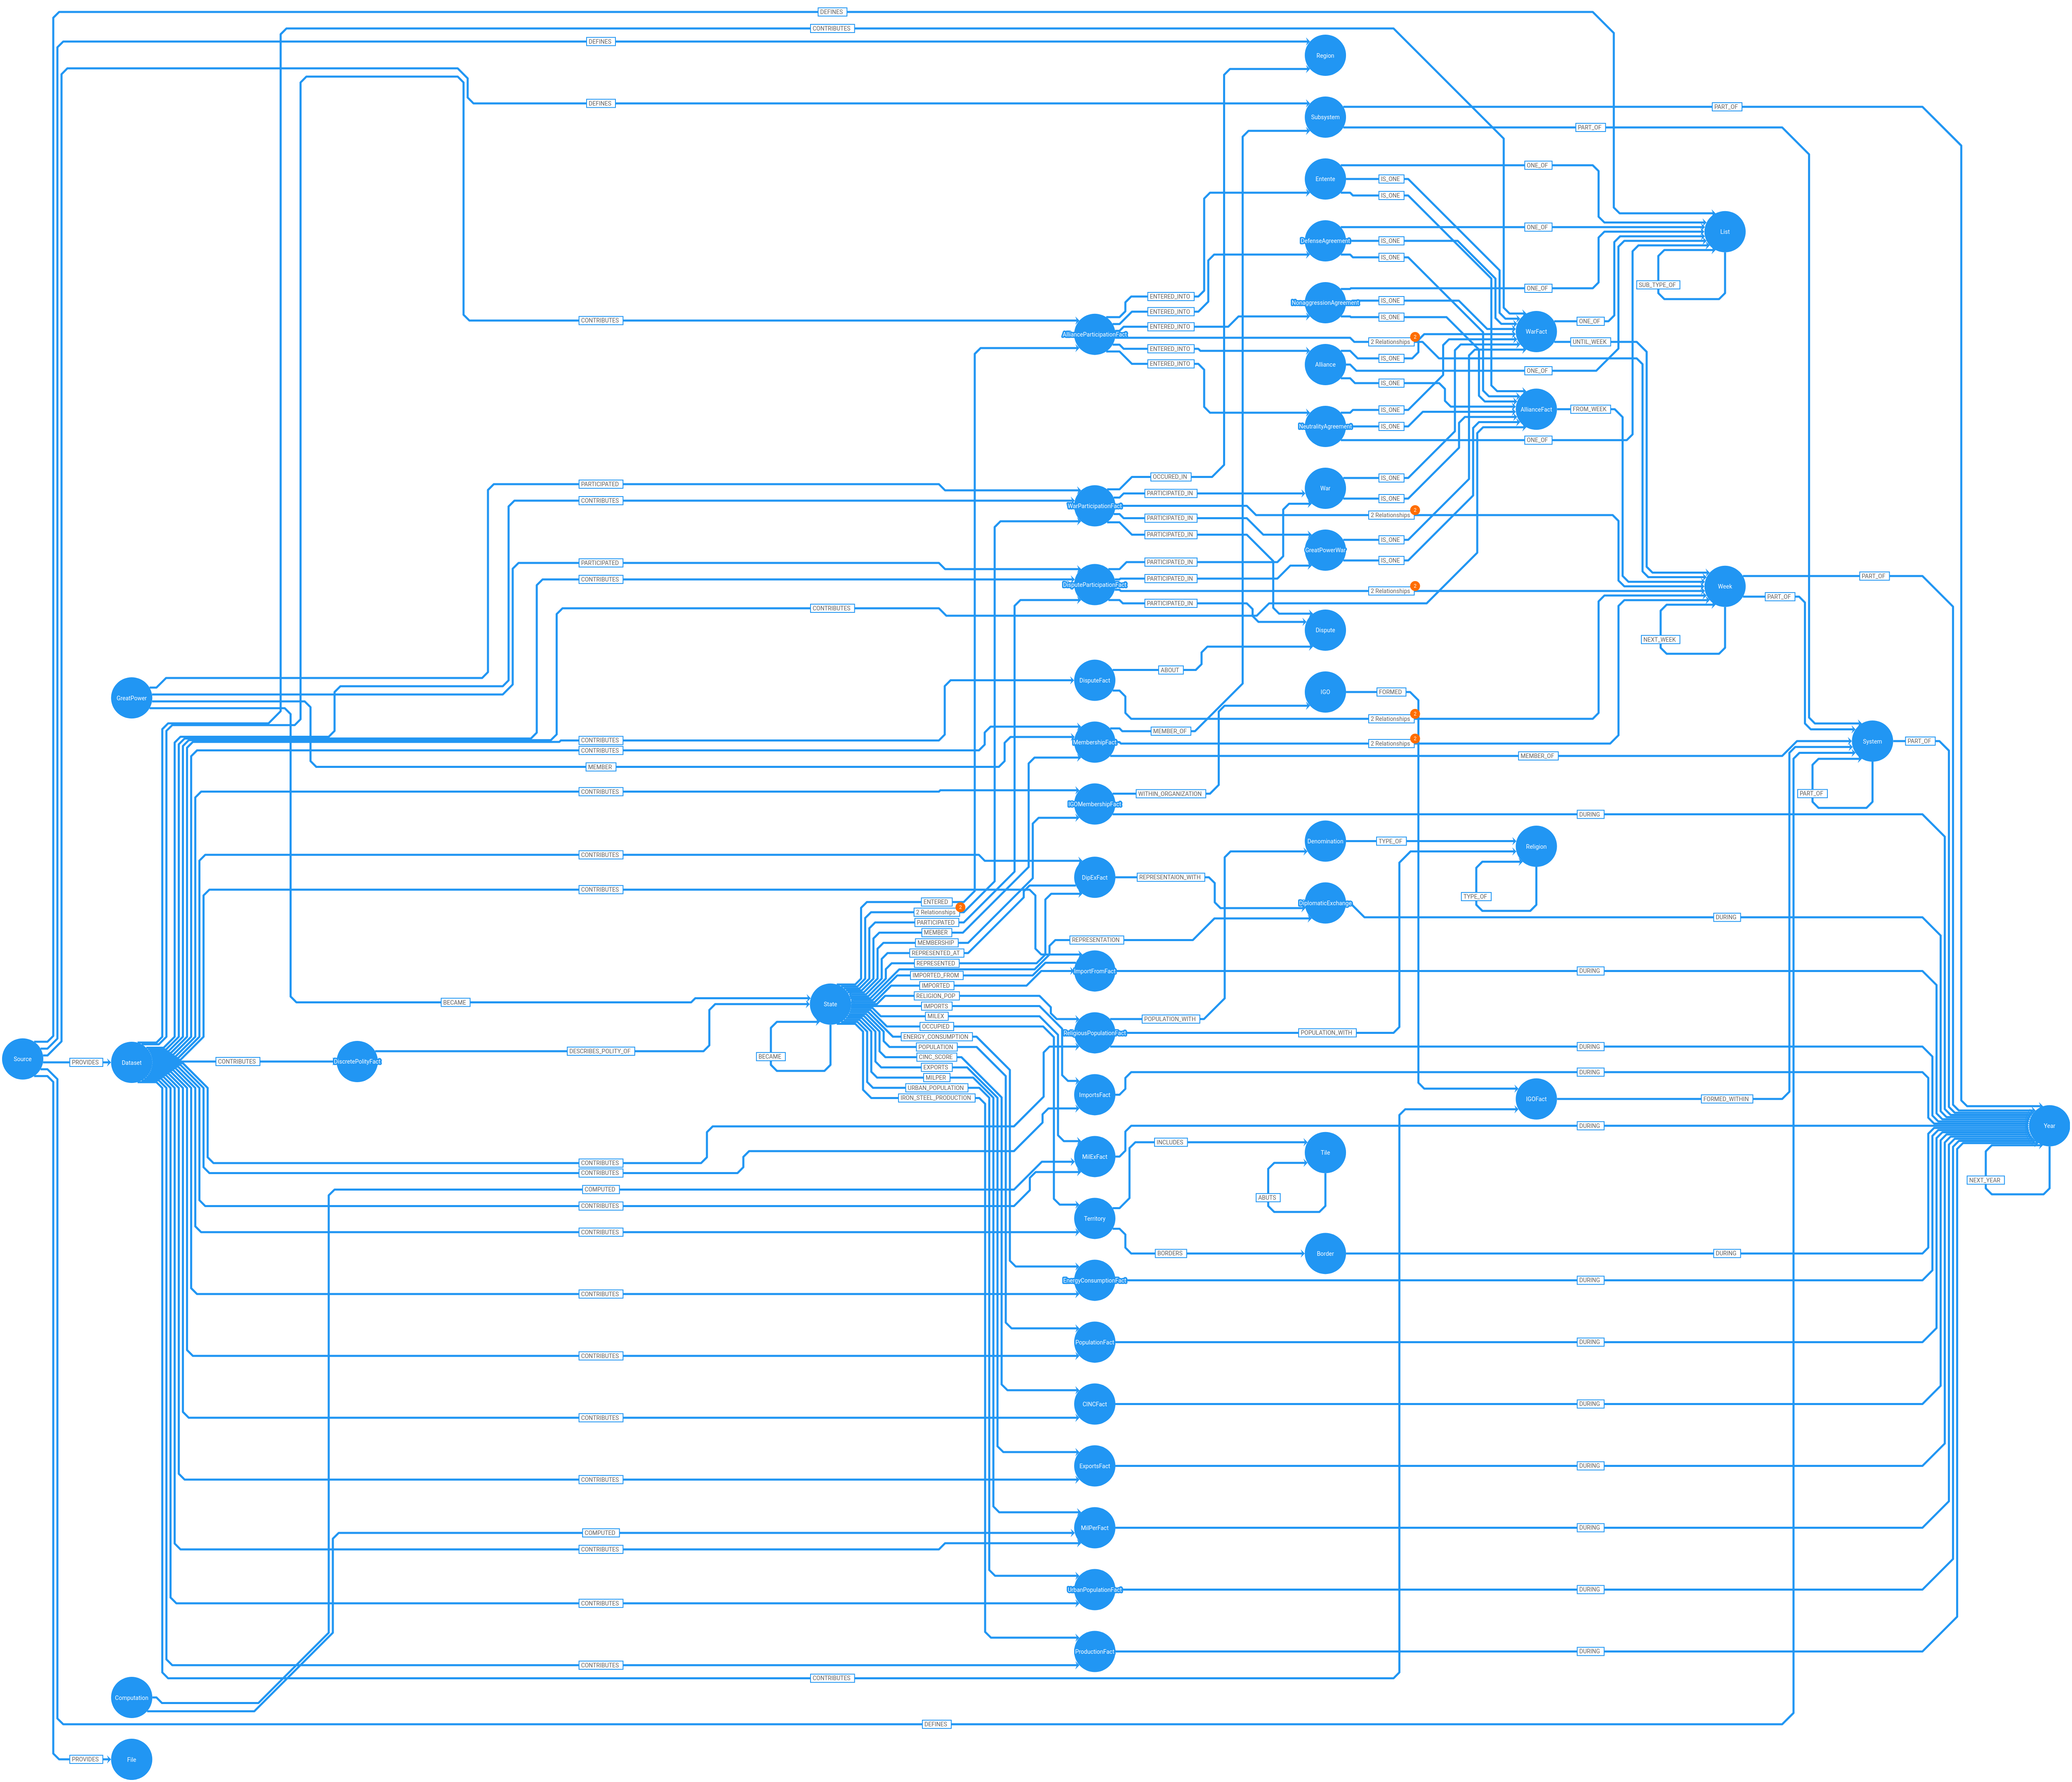
\includegraphics[width=\textwidth]{validationMetaData_yFiles.png}
\caption{Simplified meta-graph depicting the node labels and relationship types for the combined dataset.} \label{metagraph}
\end{figure}

Figure \ref{metagraph} represents a simplified meta-graph of the node labels and relationship types, revealing high-connectedness of some nodes in the data. 
The labels are much too small to read but some orientation helps to understand the resulting graph of metadata.
Importantly, the most central and most connected node represents \textit{States}. 
There are also highly connected nodes on the far left representing \textit{Datasets} and to the far right representing \textit{Years} during which events occurred or for which data is recorded. 
The nodes arranged in columns immediately to the right of the States node represent (for the most part) various \textit{Facts}: War Participation facts, System Membership facts, Territory facts, Trade facts and facts from the National Military Capabilities \cite{Singer1987} dataset, among others. 
To the right of Facts nodes are nodes that represent other system entities: \textit{Wars}, \textit{Alliances} (generally and by type), \textit{Inter-Governmental Organizations}, \textit{etc}.
It is evident in the bottom-half of the figure that many \textit{Facts} about \textit{States} relate primarily to the \textit{Years} for which they are recorded.
In the top-half of the figure, \textit{Facts} about \textit{States} are related both to these other system entities and to the \textit{Weeks} or \textit{Years} in which the relationships existed.

The graph can be queried for simple relationships as well as deep relationships and for analytical measures. 
Four useful examples follow, highlighting specific types of queries. 
The first example is simple query that asks for \textit{States} that became members of a \textit{System} between 1816 and 1825, or where the membership date is null. 
As explained in section \ref{method}, records that substitute metadata for observation dates are imported with a null value, so those missing values need to be taken into account in the query.

\begin{lstlisting}[caption={Simple relationship query.}, label={lst:simple}]
MATCH (s:State)-[m]->(mf:MembershipFact)-[mo]->(y:System) 
WHERE 1816 <= mf.from.year <=1825 OR mf.from IS NULL 
RETURN s, mf, y
\end{lstlisting}

\begin{figure}
\centering
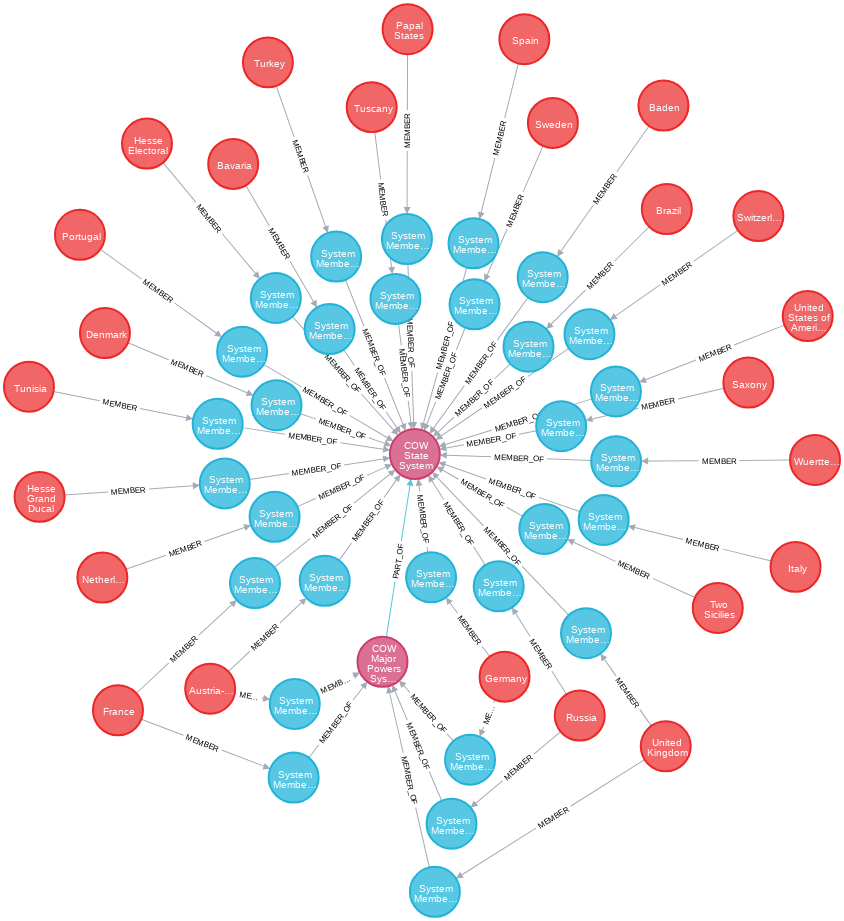
\includegraphics[width=300]{simpleMembershipGraph.png}
\caption{Example with direct relationships and filtering.} \label{simple}
\end{figure}

In this case, the database browser can be used to return results as a visualization of the relationships between \textit{States}, \textit{Facts}, and \textit{Systems}.
Because the query does not specify which system is of interest, we get results for the State System, as defined by COW project and for the Major Powers--a sub-system which is \textit{PART\_OF} the State System. 
Nodes representing \textit{States} are common to both systems but the \textit{Facts} which assert system membership uniquely mediate each relationship.

Query results can also be returned as a dataframe or table that can be used directly within a statistical computing environment.
In this example, a deep query returns all of the weeks in which a \textit{State} initiated either a war or interstate dispute and returns a dataframe with the weeks a war or dispute was initiated, the number of such events that were initiated that week, and the number of states that initiated those events.
This query was called within an \texttt{R} script that modeled the frequency that states initiated conflicts, to support a related modeling effort.

\begin{lstlisting}[caption={Deep query example}, label={lst:deep}]
MATCH (fw:Week)-[:FROM_WEEK]-(f:WarParticipationFact)-[:PARTICIPATED_IN]
  -(w:War), (f)-[p:PARTICIPATED{initiated:true}]-(s:State)
WITH collect({week:fw.stepNumber, wars:w, part:f, init:p}) AS rows
MATCH (fw:Week)-[:FROM_WEEK]-(f:DisputeParticipationFact{
  originatedDistpute:true})-[:PARTICIPATED_IN]-(d:Dispute), 
  (f)-[p:PARTICIPATED]-(s:State)
WITH rows + collect({week:fw.stepNumber, wars:d, part:f, init:p}) AS allRows
UNWIND allRows AS r
WITH r.week as week, r.wars as wars, r.part as part, r.init as init
RETURN DISTINCT week, 
  count(DISTINCT wars) as wars, 
  count(part) as states ORDER BY week
\end{lstlisting}

\begin{table}[]
\begin{center}
\caption{Conflict frequency in weeks since 1 Jan 1815 and the number of states that initiated those conflicts.}\label{tab1}
\begin{tabular}{l|l|l|l|l|l|l|l}
week    & 81    & 140   & 166   & \dots & 402   & 431   & \dots \\
\hline
wars    & 1     & 1     & 1     &       & 1     & 1     & \\
states  & 2     & 2     & 2     &       & 2     & 1     & \\
\hline
\end{tabular}
\end{center}
\end{table}

Example three is a deep query that includes spatial as well as temporal dimensions.
In a simulation, it was intended for each polity to consider which territorial neighbors and neighbors of neighbors were potential targets of military conquest while excluding partners in alliances other than peace entente. 
Agreements need be entered into prior to 1816 and not concluded before then. 

\begin{lstlisting}[caption={Spatial and temporal dimensions in queries.}, label={lst:multi}]
MATCH (t:Territory{mapKey:"Prussia of 1816"})-[:OCCUPIED]-(p1:Polity)
  -[e:ENTERED]-(apf:AllianceParticipationFact)-[:ENTERED_INTO]-(a:Alliance)
  -[:ONE_OF]-(l:List), (a)-[:ENTERED_INTO]-()-[e2:ENTERED]-(o:Polity)
WHERE e.from.year <= 1816 AND e.until.year > 1816 AND l.type <> "Entente" AND
  e2.from.year <= 1816 AND e2.until.year > 1816
WITH COLLECT(o) AS allies, t
MATCH (t)-[:BORDERS{during:1816}]->(:Border)-[:BORDERS{during:1816}]
  -(n:Territory)-[:BORDERS{during:1816}]-(:Border)-[:BORDERS{during:1816}]
  -(o:Territory)
WHERE t <> n AND t <> o
WITH COLLECT(n) + COLLECT(o) AS ter, t, allies
UNWIND ter AS z
MATCH (z)-[:OCCUPIED]-(p:Polity)
WHERE NOT p IN allies
WITH COLLECT(p) as potential
RETURN potential
\end{lstlisting}

The result for Prussia in 1816 includes 13 states: Denmark, France, Italy, the Kingdom of the Two Sicilies, the Netherlands, the Papal States, Portugal, Spain, Sweden, Switzerland, Turkey, Tuscany, and the United States of America. 

The final example calculates the betweenness centrality of territories in the 1816 map.
The query relies on two database applications that are provided with the Neo4j Desktop application: Graph Algorithms and Awesome Procedures on Cypher (APOC).
It warrants mention because it is an example of how these applications extend the capabilities of the database and the utility of the dataset.
The Graph Algorithms application can calculate the betweenness centrality of nodes in a sub-graph a single type of relationship.
However, the data model specifies \textit{Border} nodes between \textit{Territories}.

\begin{lstlisting}[caption={Territories and Borders data model.}, label={lst:model}]
(Territory)-[:BORDERS]->(Border)<-[:BORDERS]-(Territory)
\end{lstlisting}

The APOC application allows us to create ``virtual nodes'' or ``virtual relationships'' that exist as proxies within single query, even though the data does not explicitly exist in the dataset. 
Here it is used to specify a virtual relationship between \textit{Territories} via \textit{Borders} nodes and \textit{:BORDERS} relations so that the Graph Algorithms calculation of betweenness centrality can use the simplified relationship to transit the sub-graph. 

\begin{lstlisting}[caption={Query example with graph algorithm predicated on virtual relationship.}, label={lst:algo}]
CALL algo.betweenness.stream(
  'MATCH (t:Territory{year:1816}) RETURN id(t) AS id',
  'MATCH (w:Territory)-[:BORDERS{during:1816}]-(b:Border)<-
    [:BORDERS{during:1816}]-(t:Territory)  
    WHERE w<>t AND w.name <> "World Oceans" and t.name <> "World Oceans" 
    WITH t, w, apoc.create.vRelationship(w,"NEIGHBORS", {during:b.year}, t) 
    AS rel RETURN id(w) AS source, id(t) AS target',
  {graph:'cypher', write:false,  direction:'both', relationship:'rel'}
)
YIELD nodeId, centrality
MATCH (t:Territory) WHERE id(t) = nodeId
RETURN t.name AS territory, centrality ORDER BY centrality DESC
\end{lstlisting}

\begin{table}[]
\begin{center}
\caption{Betweenness centrality of five most central 1816 map territories.}\label{tab2}
\begin{tabular}{l|l}
\hline
territory & centrality \\
\hline
Russian Empire & 3791.9522 \\
Unclaimed 5 & 3721.2833 \\
Ottoman Empire & 3181.6423 \\
Egypt & 2616.6833 \\
Prussia & 1863.4437 \\
\vdots & \\
\hline
\end{tabular}
\end{center}
\end{table}

\section{Discussion\label{discussion}}
%(4-6 pages including tables, figures) Write this section second! 
%
%This section is entirely based on section 3.
The examples in \ref{results}, are intended to provide a glimpse at how data in a graph database can be extracted for use in modeling and simulation.
This section provides additional information about each of the examples in \ref{results}, above and points out the significance of those examples.
This project to collect and integrate peace science data into a graph began as an effort to support one particular research project, but has proven useful for other analysis.
The general approach used in this project may benefit other research areas with multiple, related datasets.

\subsection{Discussion of Findings}
%What do your findings mean? 
%What did you learn? 
%Answer the “so what?” question about your analysis. 
%Provide direct answers to the question(s)/puzzle(s) in section 1 (Introduction).
%What did you expect to find before you began the study? 
%What did you actually find? 
%Different? 
%Why?

The first query example at listing \ref{lst:simple} is a straight forward database filter and join operation and is a typical application of relational databases. 
It is included here to orient the reader to the Cypher query language (CQL) and point out that the basic capabilities of relational databases are available in graph databases, as well.
It also demonstrates some features of the CQL syntax. 
In this case, the query acknowledges that we expect there to be some relationship between \textit{States} and \textit{MembershipFacts} as well as between \textit{MembersipFacts} and \textit{Systems}, but it need not be specified.
The CQL `MATCH` statement is similar to a standard query language (SQL) `SELECT` statement.
The `WHERE` and `RETURN` clauses are similar in both languages.
If there were multiple sources of \textit{MembershipFacts}, such as Gleditsch's ``Extended State System Data'' \cite{Gleditsch2004} then it would be necessary to specify which sources or datasets must be related to the \textit{Facts}. 

The example at listing \ref{lst:deep} combines data from two sources: a calendar tree and the COW Inter-state War Data \cite{cow_war}.
The query searches for deeper relationships than in the first example, in that it looks first for weeks during which \textit{States} participate in armed conflict and then relates those \textit{ParticipationFacts} to the both the conflicts and the participating \textit{States}, filtering participation relationships by an `initiated` flag. 
This query also demonstrates aggregation (counts) and the `DISTINCT` key word, which simplifies further interpretation of the data, making it easier to consume in the simulation program.
Following the mediated facts data model, these results could also be filtered by the source of the data in cases when there are competing datasets or multiple versions of data available.
Again, this feature is not provided in the example.

The third query, shown in listing \ref{lst:multi} is significant, not only because it combines states with other system entities (alliances) but also with temporal and spatial dimensions of the data.
It is also a good example of when a graph database is more useful than a relation database. 
This query is selective, in that the first part of the query returns a single result (the territory occupied by Prussia in 1816).
From there, it includes eight relationships--which would have required three temporary tables and 12 joins in a relational database.
The graph database query is not only more simple to conceptualize and write, but likely executes faster; taking only 13 milliseconds over a network connection.

Listing \ref{lst:algo} for the final example demonstrates the utility of employing virtual data to represent implied relationships and uses that virtual data to calculate node properties on a sub-graph, using a common graph centrality metric. 
The Neo4j software used in this project includes seven different procedures to measure centrality, six for community detection, seven path-finding algorithms, five similarity measures, and seven link prediction algorithms. 
Advanced users can write write their own procedures if the included methods do not satisfy their specific requirements.
Using these methods is relatively easy, once the query has been correctly formulated.
The query is only eight lines long in the example, but within a simulation (where the results need not be printed out for review) is only four lines of code.

\subsection{Discussion of Broader Implications}
%Discuss the implications of your results for a broader set of ideas beyond the specific domain of analysis. Which aspects of your findings can you generalize to a larger set of patterns or cases? Interesting extentions?
The graph database used here was developed to support initialization, verification and validation of a particular agent-based simulation but it has wider utility. 
The database can be accessed with connectors for many programming languages and programming environments; Java and Python being the foremost languages used in ABM toolkits such as MASON, REPAST, or MESA and Java being the language underlying popular environments such as NetLogo and Gama where models are specified with higher-level scripts. 

The database can be accessed via statistical programming languages such as Python (again) and R.
This allows, for example, a script used in the statistical examination of an empirical dataset to be repeated directly on data collected from a simulation; thus supporting validation and study of simulation data.
In another use case, missing values from empirical data can be imputed and saved back to the database. 
By using a model where:

\begin{lstlisting}[caption={Managing provenance of computed values in a dataset.}, label={lst:compute}]
(:Dataset)-[:CONTRIBUTES]->(:Fact)<-[:COMPUTED]-(:Computation)
\end{lstlisting}

It is possible to use these computed facts within simulations and computations when desired, and exclude them when necessary.

\subsection{Implications for future research}
%How would you conduct a follow-up study? 
%Would you do things differently? 
%How so?
The data included in the dataset used in this project is limited, the spatial data has not been validated and a great deal of historical non-state data has not been included. 
Future work might expand on the available data and add competing data.
For example, Somebody \cite{missing} has published data on historical populations in African territories, which could supplant data missing in the National Military Capabilities data, which focuses on states.
Some work to integrate Gleditsch's Expanded War Data into the graph, which offers competing facts to the Correlates of War data.

There also exists an opportunity to verify published datasets when the same fact can be asserted by more than one source.
The data model used here can further be supplemented with the sources of facts in each published dataset, allowing more robust criticism, which is a necessary process in good science. 

The simulation research that this database supports is still developing and some of the implementation details of the data project will change to meet the evolving requirements of the simulation.
It is expected that the simulation of wars, peace agreements, trade volume, \textit{etc.} of each simulation run will be saved to the database with simulation run details stored as the provenance of that data.
Stored queries, such as those presented in this report, will be used to compare simulated institutional artifacts to the historical institutions represented in the data.

Mentioned in section \ref{method}, the published datasets integrated into this database are imported by script that require little or no editing of the data before importing. 
This is an important feature of this project as well as any other projects that implement this method.
Down-stream projects such as this should place no expectations on the authors who publish the source data.
Importing data by script also supports verification of the import methods and validation of the graph data representation.

\section{Conclusion\label{conclusion}} 
%(0.5-1 pages) 
%State the main problem or puzzle that motivated this investigation.
%State your major finding
%State your major implication
Collecting empirical data into a graph database has been useful in the context of the world order simulation.
Maintaining accurate metadata and the provenance of each fact within the database has proven to be a critical component of the database.
Section \ref{method} methods are not exhaustive, but present a general data model for relating metadata to facts in the source data.
Similarly, the results of various types of queries and uses of the data present a small sample of uses.

%
% the environments 'definition', 'lemma', 'proposition', 'corollary',
% 'remark', and 'example' are defined in the LLNCS documentclass as well.
%


%
% ---- Bibliography ----
%
% BibTeX users should specify bibliography style 'splncs04'.
% References will then be sorted and formatted in the correct style.
%
% \bibliographystyle{splncs04}
% \bibliography{mybibliography}
%
% For citations of references, we prefer the use of square brackets
% and consecutive numbers. Citations using labels or the author/year
% convention are also acceptable. The following bibliography provides
% a sample reference list with entries for journal
% articles~\cite{ref_article1}, an LNCS chapter~\cite{ref_lncs1}, a
% book~\cite{ref_book1}, proceedings without editors~\cite{ref_proc1},
% and a homepage~\cite{ref_url1}. Multiple citations are grouped
% \cite{ref_article1,ref_lncs1,ref_book1},
% \cite{ref_article1,ref_book1,ref_proc1,ref_url1}.

\begin{thebibliography}{8}\label{bib}
\bibitem{stata}
Stata Software. \url{https://www.stata.com/}. Last accessed 10 May 2019.

\bibitem{spss}
IBM SPSS Software. \url{https://www.ibm.com/analytics/spss-statistics-software}. Last accessed 10 May 2019.

\bibitem{neo4j}
Neo4j. \url{https://neo4j.com/}. Last accessed 10 May 2019.

\bibitem{iso8601}
International Standards Organization Date and Times Format https://www.iso.org/iso-8601-date-and-time-format.html

\bibitem{cow2016}
Correlates of War Project. 2017. ``State System Membership List, v2016.'' Online, http://correlatesofwar.org

\bibitem{cow_war}
Sarkees, Meredith Reid and Frank Wayman (2010). Resort to War: 1816 - 2007. Washington DC: CQ Press.

\bibitem{cow_mids}
Palmer, Glenn, Vito D'Orazio, Michael R. Kenwick, and Roseanne W. McManus. Forthcoming. “Updating the Militarized Interstate Dispute Data: A Response to Gibler, Miller, and Little.” International Studies Quarterly.

\bibitem{singer1987}
Singer, J. David. 1987. "Reconstructing the Correlates of War Dataset on Material Capabilities of States, 1816-1985" International Interactions, 14: 115-32.

\bibitem{maoz2013}
Zeev Maoz and Errol A. Henderson. 2013. ``The World Religion Dataset, 1945-2010: Logic, Estimates, and Trends.'' International Interactions, 39: 265-291.

\bibitem{gibler2009}
Gibler, Douglas M. 2009. International military alliances, 1648-2008. CQ Press.

\bibitem{pevehouse2004}
Pevehouse, Jon C., Timothy Nordstrom, and Kevin Warnke. 2004. ``The COW-2 International Organizations Dataset Version 2.0,'' Conflict Management and Peace Science 21:101-119.

\bibitem{barbieri2016}
Barbieri, Katherine and Omar M. G. Omar Keshk. 2016. Correlates of War Project Trade Data Set Codebook, Version 4.0. Online: http://correlatesofwar.org.

\bibitem{pol4}
Polity IV: Regime Authority Characteristics and Transition Datasets. Online, http://www.systemicpeace.org/inscrdata.html

\bibitem{gleditsch2004}
Gleditsch, Kristian Skrede 2004. 'A Revised List of Wars Between and Within Independent States, 1816-2002' International Interactions 30: 231-262

\end{thebibliography}
\end{document}
